\documentclass[11pt]{article}
\usepackage[margin=1in]{geometry}
\usepackage{booktabs,graphicx,amsmath,url,hyperref,xcolor,longtable,array,enumitem}
\usepackage[T1]{fontenc}
\hypersetup{colorlinks=true,linkcolor=blue!50!black,urlcolor=blue!50!black,citecolor=blue!50!black}
\setlist{nosep}
\newcommand{\code}[1]{\texttt{#1}}
\title{Which Rewrite Made My Model Slower?\\
\large Finding and Blaming Bad Graph Rewrites in TorchInductor --- Midterm Progress Report (S598APE)}
\author{Chidera Ibe}
\date{October 8, 2026}

\begin{document}
\maketitle

\section{Summary}
The proposal promised (a) a measurement harness that runs TorchInductor on real models with its
graph rewrites turned on and off, one at a time and in combinations, (b) an attribution tool that
takes a measured slowdown and names the rewrite, or pair of rewrites, that caused it, and (c) as a
stretch goal, learned guards. This report covers proposal items 1--5: the corpus and rewrite
switches (item 1), the measurement harness (item 2), the first batch of tests (item 3), the
interim results (item 4), and a working first version of the attribution tool (item 5).

Everything described here exists as code in the \code{rewrite\_blame} package, is driven from a
command line, and is exercised by 100 %
automated tests that pass on both
machines used. The main findings so far:
\begin{itemize}
\item TorchInductor~2.14.1 exposes \textbf{227 individually switchable pattern-matcher rules} plus
  26 configuration flags and 16 opt-in rewrite passes, for a universe of 269 switches. Each pattern
  rule is switched without modifying PyTorch, by wrapping the rule's \code{extra\_check} hook, and the
  harness records how often each rule fired or was suppressed in every compile.
\item The attribution tool, delta debugging over \emph{signed} switch changes with a timing judge,
  recovers planted culprits in all tests, including a genuine \textbf{pair interaction} that exists
  in Inductor today: attention-fusion rules 11 and 12 match the same graph, so disabling either one
  alone changes nothing, and only disabling both changes the compiled program (Section~\ref{sec:attr}).
\item On the models measured so far, most individual rewrites do not change the generated program
  at all (Section~\ref{sec:results}); the ones that do are the pattern rules that actually fire,
  the master pass switches, freezing, and a handful of scheduler knobs. This is useful: the
  attribution search only has to consider the rules that fired, which is a short list per model.
\end{itemize}

\paragraph{One deviation from the proposal.} No GPU was available (neither the course VM nor my
laptop has one), so every measurement in this report uses Inductor's \textbf{CPU C++/OpenMP backend}
rather than Triton. The rewrite passes under study (joint-graph, post-grad, pre-grad pattern
matching, decompositions, freezing) are the same on both backends; what differs is the kernel
generator. The code-statistics module parses both the C++ and the Triton wrapper formats and is
unit-tested against both, so a GPU run later is a change of device, not of tooling. Two very
different CPUs (an Apple M4 Pro and an x86 Xeon with AVX-512 and oneDNN) stand in for the
proposal's ``two GPUs'' repeatability check.

\section{What was built}
\subsection{Rewrite switches (proposal item 1b)}
Inductor applies its rewrites in three places: \emph{pre-grad} FX passes on the captured graph,
\emph{joint-graph} passes after AOTAutograd, and \emph{post-grad} passes before lowering; most of
them are instances of a generic \code{PatternMatcherPass}, each holding a list of
\code{PatternEntry} rules keyed by the operator they match. Reading the source showed that the pass
applies a rule only if \code{entry.extra\_check(match)} returns true. The harness therefore
replaces each entry's \code{extra\_check} with a small gate object that (1) refuses the match when
the rule's switch is off, (2) counts a \emph{fire} when the rule's own check accepts and the switch
is on, and (3) counts a \emph{suppression} when the rule would have fired but was disabled. No
PyTorch source is modified.

Rules are registered lazily, so discovery first compiles a tiny warm-up graph that touches
attention, convolution/batch-norm, split/cat, matmul and dtype casts, then walks the
\code{fx\_passes} modules for every pass object and gates every entry. Rule names come from the
entry's handler function or the replacement's \code{pattern\_name}
(e.g.\ \code{joint/joint\_graph.patterns/\_sfdp\_pattern\_11\_inference},
\code{post\_grad/pass\_patterns[1]/reciprocal\_sqrt\_to\_rsqrt}). Three further kinds of switch cover
rewrites that are not pattern entries: configuration flags (\code{epilogue\_fusion},
\code{reorder\_for\_locality}, \code{freezing}, \code{cpp.weight\_prepack}, \ldots), opt-in
``optimus'' passes enabled through Inductor's fusion-option dictionaries (split/cat normalisation,
\code{decompose\_mm\_pass}, batch fusions), and master switches for whole pass groups. A
\emph{state} is the set of switches that are on; \code{default} reproduces Inductor's behaviour.

Two details mattered for correctness. First, Inductor's on-disk FX-graph cache is keyed by its
configuration but not by pattern state; a cache hit also skips every pass, which hides which rules
fired. The harness therefore adds a no-op custom pass whose \code{uuid()} hashes the switch state
into the cache key, and disables the FX-graph cache during measurements (the generated C++ kernels
are still cached by source hash, so recompiles cost seconds). Second, calling Inductor's lazy
initialisers directly poisons their \code{functools.cache} keys and produces ``duplicate pattern''
errors on the next real compile; discovery must go through a real compile.

\subsection{Measurement harness (item 2)}
One measurement is one model under one state in a fresh subprocess, so gates, lazy state and
allocator state never leak between configurations. The worker compiles the model with
\code{torch.compile}, captures the generated wrapper code, and records:
\begin{itemize}
\item \textbf{generated-code statistics}: number of fused kernels (\code{cpp\_fused\_*} or
  \code{triton\_*}), per-kernel input/output/in-place pointer counts, static load and store sites,
  vectorisation, kernel category (pointwise/reduction), extern and fallback calls
  (\code{extern\_kernels.mm}, \code{aten.\_scaled\_dot\_product\_flash\_attention\_for\_cpu}, oneDNN
  fused convolutions), and the bytes of intermediate buffers allocated in the wrapper
  (the ``extra tensor written to memory'' the proposal worries about);
\item \textbf{Inductor's own metrics} (bytes accessed, IR nodes before fusion, loop reorderings) and
  the \code{counters["inductor"]} deltas;
\item \textbf{which rules fired or were suppressed} and the post-grad op histogram, used to verify
  that a switch really changed the graph;
\item \textbf{correctness} against eager execution (\code{allclose}, rtol/atol $10^{-3}$) under every
  state, so a ``fast'' configuration is never a wrong one;
\item \textbf{time}: fixed thread count, 10 warm-up calls, then $5\times10$ timed calls with
  per-call medians, MAD, and percentiles.
\end{itemize}
Results are stored in SQLite keyed by model, machine fingerprint, state hash and timing protocol,
so attribution never measures the same configuration twice; re-running an attribution is served
entirely from the store.

\paragraph{Noise threshold.} The baseline state is measured in seven separate processes. The
slowdown threshold is $\tau=\max(3\cdot\mathrm{MAD}(\text{medians}),\;1\%\ \text{of the centre})$;
the report also records the largest difference seen between two \emph{identical} runs, which is the
false-positive scale the threshold must exceed. Table~\ref{tab:noise} lists the measured values.

\subsection{Attribution tool (item 5, started)}\label{sec:attr-method}
Given a fast state $F$ and a slow state $S$, the candidate causes are the signed changes that turn
$F$ into $S$ (\code{+id} = turn on, \code{-id} = turn off); this covers both ``a new rewrite
hurt'' and ``a rewrite that used to help was lost''. The tool runs Zeller and Hildebrandt's
\emph{ddmin} over that change set. The judge says \emph{slow} when the median time of $F$ with the
candidate changes applied exceeds the fast reference by more than $\tau$; a candidate landing within
$\pm50\%$ of $\tau$ is measured once more and the two medians averaged. The result is 1-minimal:
removing any single culprit makes the slowdown disappear. A pair check then measures each culprit
alone and reports an \emph{interaction} when none reproduces the slowdown by itself. The report
names the culprits and prints the kernel-level difference between $F$ and $F$+culprits: kernel
count and names, extern calls, intermediate bytes, and which rules changed their firing. A
second judge type uses a deterministic compile-time metric (kernel count, allocation bytes) and is
what the tests on planted slowdowns use, so they are immune to timing noise.

\subsection{Model corpus (item 1a)}
Table~\ref{tab:corpus} lists the 24 %
registered models: six hand-written
graphs that each plant one rewrite family, six torchvision models, and twelve HuggingFace
configurations including LLM prefill and single-token (decode) shapes. Models are built from fixed
configs with random weights, so nothing is downloaded and timings do not depend on weights. Decode
graphs are single-token forwards without a KV cache for now.

\section{Testing (item 3)}
Tests are split into \emph{unit} tests (no compilation; \code{tests/test\_u\_*.py}) and
\emph{Inductor} tests that compile small graphs (\code{tests/test\_i\_*.py}); Table~\ref{tab:tests}
counts them. Highlights:
\begin{itemize}
\item \textbf{ddmin on synthetic cost models}: single culprit, pair-only culprit (flagged as an
  interaction), two independent culprits (1-minimal result), three-way interaction, a masking
  rewrite that speeds up, a noisy judge (18/20 seeds correct at $\tau = 3\sigma$), 25 random cost
  models checked for ``slow and 1-minimal'', memoisation, and the logarithmic number of judge calls
  (a culprit among 256 changes in $\le 40$ evaluations).
\item \textbf{counters}: the code-statistics parser on hand-written C++ and Triton wrapper fixtures
  with known kernel counts, pointer counts, loads/stores, extern calls, allocation bytes including
  a symbolic shape, and the diff that ignores kernel numbering.
\item \textbf{noise threshold}: MAD with floor, quiet-machine floor, re-measure band of the timing
  judge, serialisation.
\item \textbf{planted rewrites} (compiled): for each toy graph, the expected rule fires by default,
  its switch suppresses it, the post-grad graph changes in the predicted way (e.g.\ \code{rsqrt}
  becomes \code{sqrt}+\code{reciprocal}; the dtype round trip survives without
  \code{pointless\_convert}; SDPA disappears and two \code{bmm} calls plus a softmax kernel appear
  without the attention rules; \code{decompose\_mm\_pass} removes \code{mm} calls on the decode MLP;
  freezing folds batch-norm into the convolutions), and outputs match eager under both states.
\item \textbf{pipeline}: subprocess isolation, store caching (second call makes no new measurement),
  failure reporting, the planted sfdp \{11,12\} interaction recovered by attribution with a metric
  judge in fewer compiles than leave-one-out, a single config culprit hidden among no-op changes,
  switch-effect classification, and determinism of the switch registry across processes.
\end{itemize}

\begin{table}[h]\centering\small
\begin{tabular}{lr}\toprule test file & tests \\\midrule
test\_i\_discover.py & 17 \\
test\_i\_pipeline.py & 9 \\
test\_i\_planted.py & 9 \\
test\_u\_attribute.py & 40 \\
test\_u\_codegen\_stats.py & 6 \\
test\_u\_judge\_stats.py & 8 \\
test\_u\_store.py & 3 \\
test\_u\_switches.py & 8 \\
\textbf{total} & \textbf{100} \\%

\bottomrule\end{tabular}
\caption{Automated tests (unit tests run in well under a second; Inductor tests compile toy graphs).}\label{tab:tests}
\end{table}

\section{Results so far (item 4)}\label{sec:results}

\subsection{Noise}
\begin{table}[h]\centering\small
\begin{tabular}{llrrrrrr}\toprule
model & machine & runs & centre (ms) & MAD (ms) & $\tau$ (ms) & $\tau$ (\%) & max $|\Delta|$ identical (ms) \\\midrule
attention\_block & Mac & 7 & 0.926 & 0.006 & 0.017 & 1.8 & 0.029 \\
bert\_base\_eagerattn & Mac & 7 & 84.363 & 0.968 & 2.905 & 3.4 & 1.708 \\
decode\_mlp & Mac & 7 & 0.194 & 0.004 & 0.011 & 5.5 & 0.046 \\
gpt2\_prefill & Mac & 7 & 62.447 & 0.600 & 1.800 & 2.9 & 1.125 \\
norm\_mlp & Mac & 7 & 1.058 & 0.006 & 0.018 & 1.7 & 0.047 \\
resnet18 & Mac & 7 & 26.118 & 0.192 & 0.576 & 2.2 & 0.451 \\
attention\_block & VM & 7 & 8.526 & 0.066 & 0.198 & 2.3 & 0.320 \\
norm\_mlp & VM & 7 & 12.478 & 0.052 & 0.155 & 1.2 & 1.660 \\%

\bottomrule\end{tabular}
\caption{Baseline noise from repeated identical runs in separate processes. ``mac'' is the Apple M4
Pro (8 threads), ``fa26'' the course VM (4-core Xeon Silver 4216).}\label{tab:noise}
\end{table}
\begin{figure}[h]\centering
\IfFileExists{figures/noise.pdf}{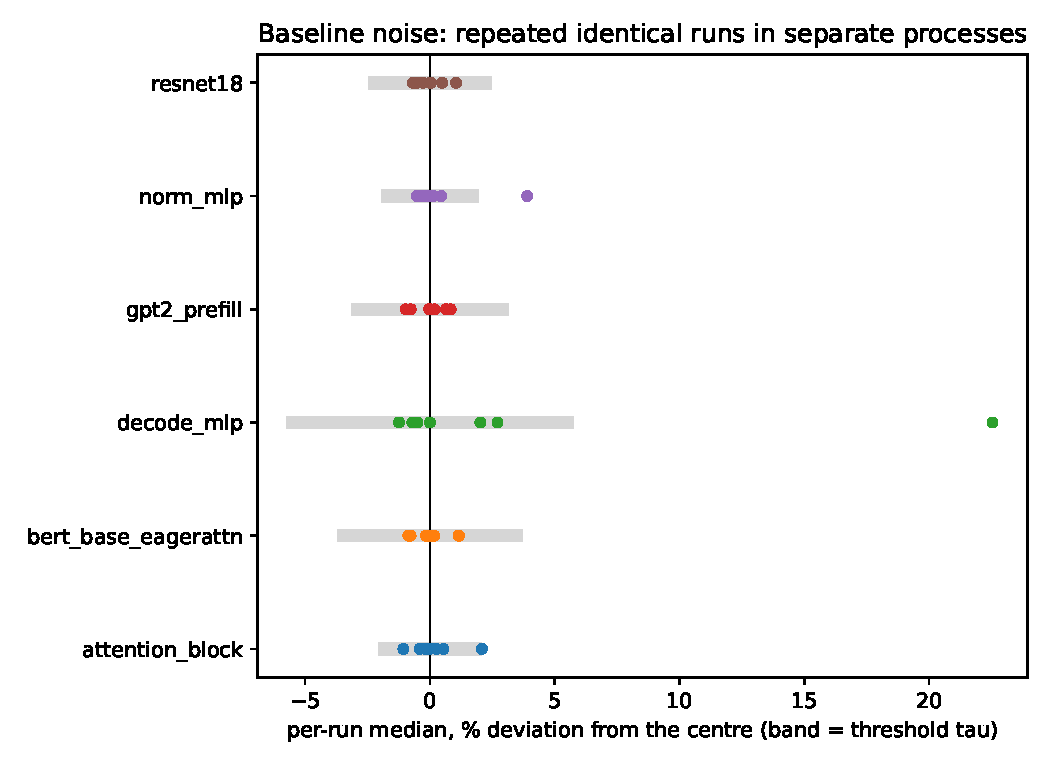
\includegraphics[width=0.85\linewidth]{figures/noise.pdf}}{\fbox{noise.pdf pending}}
\caption{Per-run medians of identical baseline runs, as deviation from the centre; the grey band is $\tau$.}
\end{figure}

\subsection{Does flipping a switch change the program?}
For each model the harness compiles the default state, then toggles every candidate switch (every
rule that fired, every config flag, every opt-in option) and classifies the effect:
\emph{changes graph} (different kernels, extern calls, allocation or post-grad ops),
\emph{fires only} (a different rule fired but the program is the same), or \emph{no effect}.
\begin{table}[h]\centering\small
\begin{tabular}{lrrlrrrr}\toprule
model & kernels & rules fired & candidates (pat/cfg/opt) & changes graph & fires only & no effect & errors \\\midrule
attention\_block & 1 & 4 & 4/26/16 & 5 & 6 & 35 & 0 \\
decode\_mlp & 1 & 0 & 0/26/16 & 4 & 0 & 38 & 0 \\
norm\_mlp & 3 & 4 & 4/26/16 & 8 & 2 & 36 & 0 \\
resnet18 & 14 & 1 & 1/26/16 & 4 & 3 & 36 & 0 \\%

\bottomrule\end{tabular}
\caption{Switch verification. A pattern rule that never fired cannot change anything when turned
off, so only fired rules are candidates.}\label{tab:verify}
\end{table}

\subsection{Leave-one-out timing sweeps}
\subsubsection*{attention\_block on the Mac (M4 Pro, 8 threads)}
Baseline 0.926~ms, $\tau$ = 0.017~ms (1.8\%). 5 graph-changing switches were toggled one at a time: 2 made the model slower than $\tau$, 0 made it faster, 3 stayed within noise. Slower: \code{master/pattern\_matcher} (off, +33.1\%); \code{master/post\_grad\_passes} (off, +3.2\%). 
\begin{table}[h]\centering\scriptsize
\begin{tabular}{llrrrl}\toprule
switch & toggled & median (ms) & $\Delta$ (\%) & kernels & vs.\ $\tau$ \\\midrule
master/pattern\_matcher & off & 1.232 & +33.1 & 4 & \textbf{slower} \\
master/post\_grad\_passes & off & 0.955 & +3.2 & 2 & \textbf{slower} \\
optimus/normalization\_pass & on & 0.916 & -1.1 & 1 &  \\
sched/inplace\_buffers & off & 0.928 & +0.3 & 1 &  \\
lowering/freezing & on & 0.925 & -0.0 & 1 &  \\
\bottomrule\end{tabular}
\caption{Leave-one-out sweep, attention\_block, Mac (M4 Pro, 8 threads).}
\end{table}
\IfFileExists{figures/sweep_attention_block.pdf}{\begin{figure}[h]\centering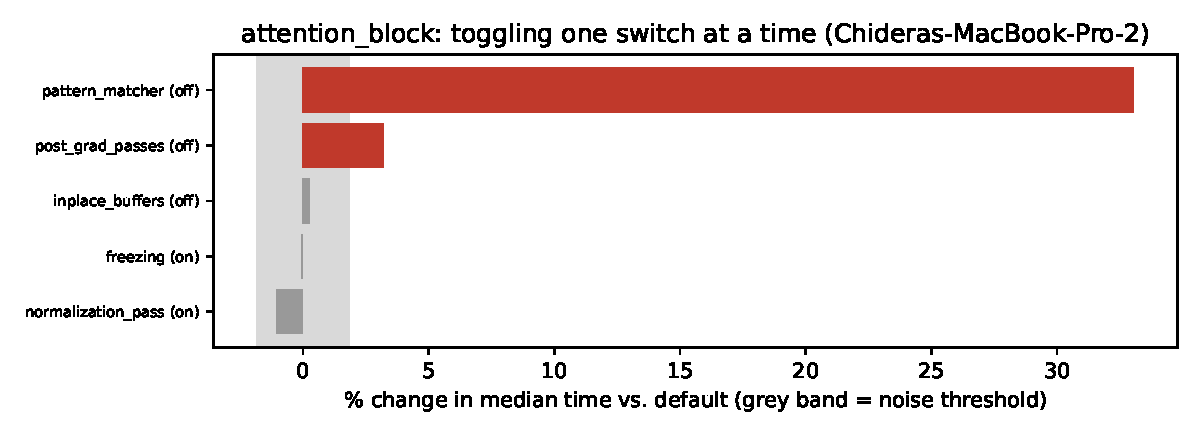
\includegraphics[width=0.9\linewidth]{figures/sweep_attention_block.pdf}\end{figure}}{}

\subsubsection*{decode\_mlp on the Mac (M4 Pro, 8 threads)}
Baseline 0.194~ms, $\tau$ = 0.011~ms (5.5\%). 4 graph-changing switches were toggled one at a time: 1 made the model slower than $\tau$, 0 made it faster, 3 stayed within noise. Slower: \code{optimus/decompose\_mm\_pass} (on, +15.0\%). 
\begin{table}[h]\centering\scriptsize
\begin{tabular}{llrrrl}\toprule
switch & toggled & median (ms) & $\Delta$ (\%) & kernels & vs.\ $\tau$ \\\midrule
optimus/decompose\_mm\_pass & on & 0.223 & +15.0 & 1 & \textbf{slower} \\
master/post\_grad\_passes & off & 0.191 & -1.6 & 1 &  \\
lowering/freezing & on & 0.191 & -1.4 & 1 &  \\
sched/inplace\_buffers & off & 0.191 & -1.1 & 1 &  \\
\bottomrule\end{tabular}
\caption{Leave-one-out sweep, decode\_mlp, Mac (M4 Pro, 8 threads).}
\end{table}
\IfFileExists{figures/sweep_decode_mlp.pdf}{\begin{figure}[h]\centering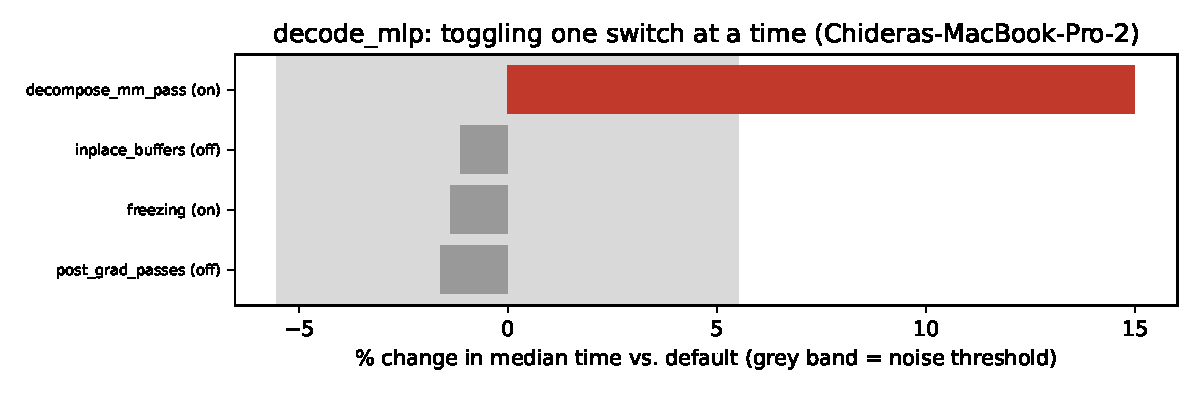
\includegraphics[width=0.9\linewidth]{figures/sweep_decode_mlp.pdf}\end{figure}}{}

\subsubsection*{norm\_mlp on the Mac (M4 Pro, 8 threads)}
Baseline 1.058~ms, $\tau$ = 0.018~ms (1.7\%). 8 graph-changing switches were toggled one at a time: 2 made the model slower than $\tau$, 0 made it faster, 6 stayed within noise. Slower: \code{sched/inplace\_buffers} (off, +4.3\%); \code{joint/constant\_folding} (off, +2.6\%). 
\begin{table}[h]\centering\scriptsize
\begin{tabular}{llrrrl}\toprule
switch & toggled & median (ms) & $\Delta$ (\%) & kernels & vs.\ $\tau$ \\\midrule
sched/inplace\_buffers & off & 1.103 & +4.3 & 3 & \textbf{slower} \\
joint/constant\_folding & off & 1.085 & +2.6 & 3 & \textbf{slower} \\
master/post\_grad\_passes & off & 1.067 & +0.9 & 3 &  \\
pointless\_view\_pair & off & 1.065 & +0.7 & 3 &  \\
lowering/freezing & on & 1.052 & -0.5 & 3 &  \\
master/pattern\_matcher & off & 1.062 & +0.4 & 3 &  \\
pointless\_convert & off & 1.059 & +0.2 & 3 &  \\
reciprocal\_sqrt\_to\_rsqrt & off & 1.058 & +0.0 & 3 &  \\
\bottomrule\end{tabular}
\caption{Leave-one-out sweep, norm\_mlp, Mac (M4 Pro, 8 threads).}
\end{table}
\IfFileExists{figures/sweep_norm_mlp.pdf}{\begin{figure}[h]\centering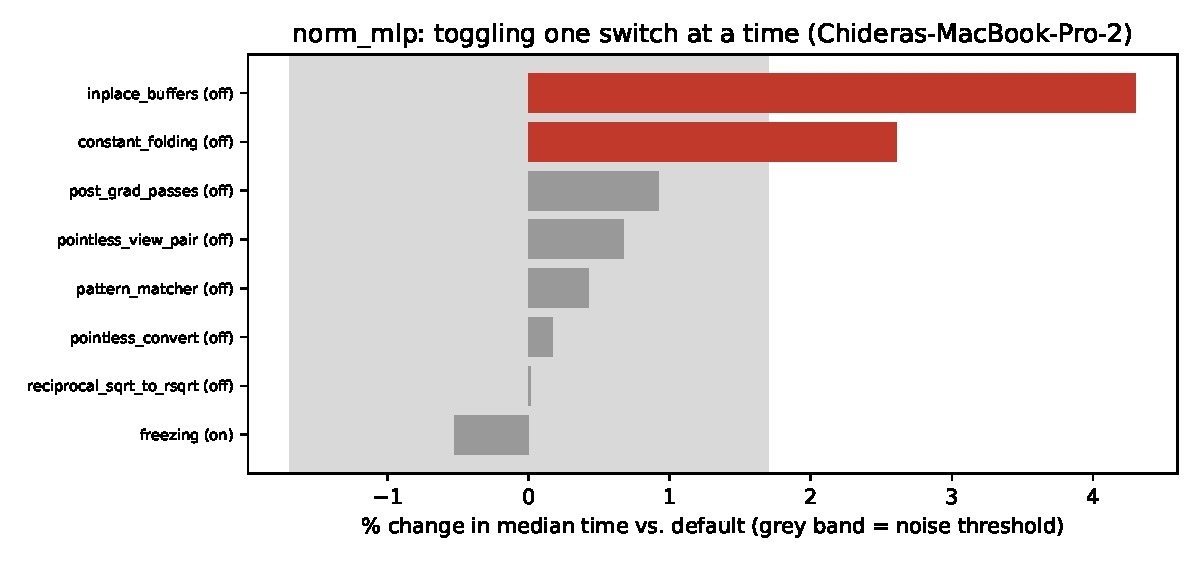
\includegraphics[width=0.9\linewidth]{figures/sweep_norm_mlp.pdf}\end{figure}}{}

\subsubsection*{resnet18 on the Mac (M4 Pro, 8 threads)}
Baseline 26.118~ms, $\tau$ = 0.576~ms (2.2\%). 4 graph-changing switches were toggled one at a time: 1 made the model slower than $\tau$, 0 made it faster, 3 stayed within noise. Slower: \code{lowering/layout\_optimization} (off, +11.1\%). 
\begin{table}[h]\centering\scriptsize
\begin{tabular}{llrrrl}\toprule
switch & toggled & median (ms) & $\Delta$ (\%) & kernels & vs.\ $\tau$ \\\midrule
lowering/layout\_optimization & off & 29.007 & +11.1 & 12 & \textbf{slower} \\
lowering/freezing & on & 25.827 & -1.1 & 11 &  \\
sched/inplace\_buffers & off & 26.239 & +0.5 & 14 &  \\
master/post\_grad\_passes & off & 26.099 & -0.1 & 14 &  \\
\bottomrule\end{tabular}
\caption{Leave-one-out sweep, resnet18, Mac (M4 Pro, 8 threads).}
\end{table}
\IfFileExists{figures/sweep_resnet18.pdf}{\begin{figure}[h]\centering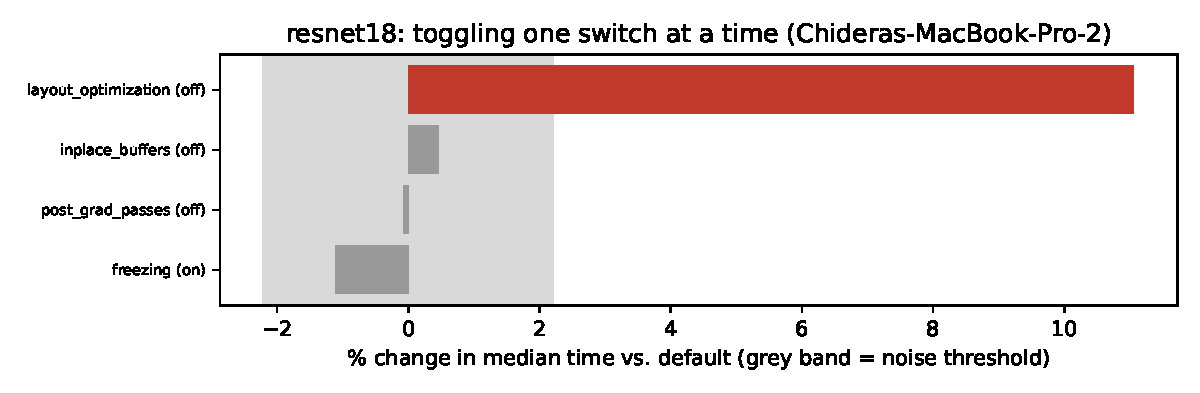
\includegraphics[width=0.9\linewidth]{figures/sweep_resnet18.pdf}\end{figure}}{}%


\section{Attribution case studies}\label{sec:attr}
\subsection*{attention\_block on the Mac (M4 Pro, 8 threads): verdict \emph{interaction}}
The slow state differs from the fast state in 63 switches. Fast 0.919~ms vs.\ slow 1.250~ms (+36.1\%); $\tau$ = 0.017~ms. ddmin needed 16 judge evaluations (versus 63 for leave-one-out, 1953 for all pairs) and returned the culprit set \code{-joint/joint\_\allowbreak{}graph.\allowbreak{}patterns/\_\allowbreak{}sfdp\_\allowbreak{}pattern\_\allowbreak{}11\_\allowbreak{}inference}, \code{-joint/joint\_\allowbreak{}graph.\allowbreak{}patterns/\_\allowbreak{}sfdp\_\allowbreak{}pattern\_\allowbreak{}12\_\allowbreak{}inference}. Each culprit alone was judged \emph{fast}: the slowdown needs all of them together. \textbf{Kernel-level explanation.} fused kernels 1 $\rightarrow$ 4, extern calls 3 $\rightarrow$ 4, intermediate bytes 4,198,400 $\rightarrow$ 11,591,680. Kernels gained: \code{cpp\_\allowbreak{}fused\_\allowbreak{}\_\allowbreak{}softmax\_\allowbreak{}abs\_\allowbreak{}all\_\allowbreak{}amax\_\allowbreak{}div\_\allowbreak{}eq\_\allowbreak{}mul\_\allowbreak{}ne\_\allowbreak{}sub\_\allowbreak{}view}, \code{cpp\_\allowbreak{}fused\_\allowbreak{}clone\_\allowbreak{}split\_\allowbreak{}transpose\_\allowbreak{}view}, \code{cpp\_\allowbreak{}fused\_\allowbreak{}clone\_\allowbreak{}transpose\_\allowbreak{}view}. Extern calls lost: \code{torch.\allowbreak{}ops.\allowbreak{}aten.\allowbreak{}\_\allowbreak{}scaled\_\allowbreak{}dot\_\allowbreak{}product\_\allowbreak{}flash\_\allowbreak{}attention\_\allowbreak{}for\_\allowbreak{}cpu}; gained: \code{extern\_\allowbreak{}kernels.\allowbreak{}bmm} ($\times$2). Rules suppressed in the culprit state: \code{\_\allowbreak{}sfdp\_\allowbreak{}pattern\_\allowbreak{}11\_\allowbreak{}inference}, \code{\_\allowbreak{}sfdp\_\allowbreak{}pattern\_\allowbreak{}12\_\allowbreak{}inference}. 
\begin{table}[h]\centering\small
\begin{tabular}{lp{0.62\linewidth}}\toprule
field & value \\\midrule
\textbf{model} & attention\_block (Chideras-MacBook-Pro-2) \\
judge & timing (median\_ms) \\
fast reference & 0.926 ms, $\tau$ = 0.017 ms (1.8\%) \\
slow state & 1.250 ms \\
candidate changes & 63 \\
judge evaluations & 16 \\
verdict & interaction \\
culprits & \code{\_\allowbreak{}sfdp\_\allowbreak{}pattern\_\allowbreak{}11\_\allowbreak{}inference}, \code{\_\allowbreak{}sfdp\_\allowbreak{}pattern\_\allowbreak{}12\_\allowbreak{}inference} \\
kernels fast $\rightarrow$ culprits & 1 $\rightarrow$ 4 \\
extern calls & 3 $\rightarrow$ 4 \\
intermediate bytes & 4,198,400 $\rightarrow$ 11,591,680 \\
median ms & 0.919 $\rightarrow$ 1.244 \\
\bottomrule\end{tabular}
\caption{Attribution summary, attention\_block.}
\end{table}
\IfFileExists{figures/trace_attention_block_mac.pdf}{\begin{figure}[h]\centering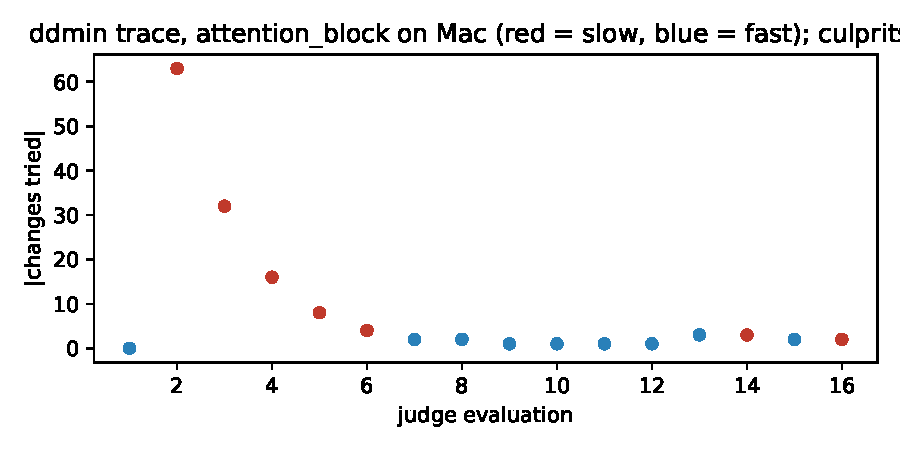
\includegraphics[width=0.7\linewidth]{figures/trace_attention_block_mac.pdf}\caption{ddmin search trace for attention\_block (Mac (M4 Pro, 8 threads)): each point is one judge evaluation.}\end{figure}}{}

\subsection*{decode\_mlp on the Mac (M4 Pro, 8 threads): verdict \emph{single}}
The slow state differs from the fast state in 16 switches. Fast 0.195~ms vs.\ slow 0.222~ms (+14.1\%); $\tau$ = 0.011~ms. ddmin needed 7 judge evaluations (versus 16 for leave-one-out, 120 for all pairs) and returned the culprit set \code{+optimus/decompose\_\allowbreak{}mm\_\allowbreak{}pass}. A single change reproduces the whole slowdown. \textbf{Kernel-level explanation.} fused kernels 1 $\rightarrow$ 1, extern calls 3 $\rightarrow$ 0, intermediate bytes 20,480 $\rightarrow$ 20,480. Kernels lost: \code{cpp\_\allowbreak{}fused\_\allowbreak{}mul\_\allowbreak{}silu}. Kernels gained: \code{cpp\_\allowbreak{}fused\_\allowbreak{}mm\_\allowbreak{}mul\_\allowbreak{}silu\_\allowbreak{}t}. Extern calls lost: \code{extern\_\allowbreak{}kernels.\allowbreak{}mm} ($\times$3); gained: none. 
\begin{table}[h]\centering\small
\begin{tabular}{lp{0.62\linewidth}}\toprule
field & value \\\midrule
\textbf{model} & decode\_mlp (Chideras-MacBook-Pro-2) \\
judge & timing (median\_ms) \\
fast reference & 0.194 ms, $\tau$ = 0.011 ms (5.5\%) \\
slow state & 0.222 ms \\
candidate changes & 16 \\
judge evaluations & 7 \\
verdict & single \\
culprits & \code{+optimus/decompose\_\allowbreak{}mm\_\allowbreak{}pass} \\
kernels fast $\rightarrow$ culprits & 1 $\rightarrow$ 1 \\
extern calls & 3 $\rightarrow$ 0 \\
intermediate bytes & 20,480 $\rightarrow$ 20,480 \\
median ms & 0.195 $\rightarrow$ 0.223 \\
\bottomrule\end{tabular}
\caption{Attribution summary, decode\_mlp.}
\end{table}
\IfFileExists{figures/trace_decode_mlp_mac.pdf}{\begin{figure}[h]\centering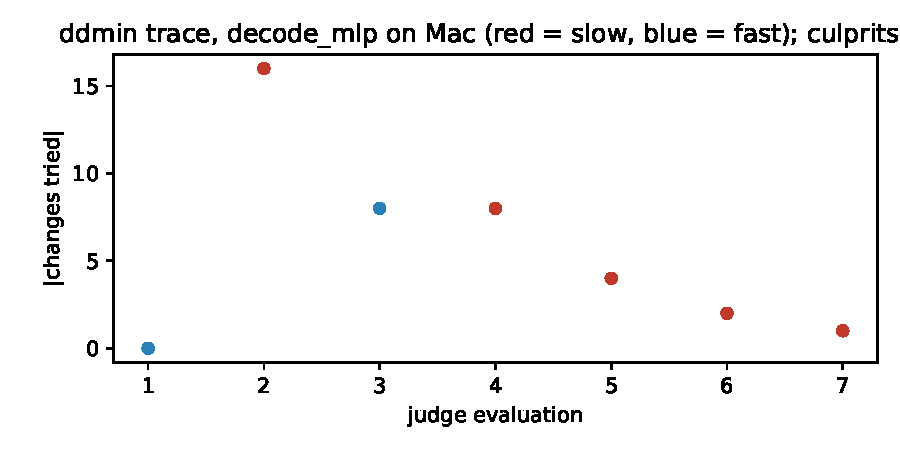
\includegraphics[width=0.7\linewidth]{figures/trace_decode_mlp_mac.pdf}\caption{ddmin search trace for decode\_mlp (Mac (M4 Pro, 8 threads)): each point is one judge evaluation.}\end{figure}}{}

\subsection*{norm\_mlp on the Mac (M4 Pro, 8 threads): verdict \emph{single}}
The slow state differs from the fast state in 8 switches. Fast 1.061~ms vs.\ slow 1.099~ms (+3.6\%); $\tau$ = 0.018~ms. ddmin needed 8 judge evaluations (versus 8 for leave-one-out, 28 for all pairs) and returned the culprit set \code{-joint/constant\_\allowbreak{}folding}. A single change reproduces the whole slowdown. \textbf{Kernel-level explanation.} fused kernels 3 $\rightarrow$ 3, extern calls 2 $\rightarrow$ 2, intermediate bytes 1,573,376 $\rightarrow$ 1,573,376. Kernels lost: \code{cpp\_\allowbreak{}fused\_\allowbreak{}add\_\allowbreak{}gelu\_\allowbreak{}mean\_\allowbreak{}mul\_\allowbreak{}pow}. Kernels gained: \code{cpp\_\allowbreak{}fused\_\allowbreak{}add\_\allowbreak{}gelu\_\allowbreak{}mean\_\allowbreak{}mul\_\allowbreak{}pow\_\allowbreak{}reciprocal}. 
\begin{table}[h]\centering\small
\begin{tabular}{lp{0.62\linewidth}}\toprule
field & value \\\midrule
\textbf{model} & norm\_mlp (Chideras-MacBook-Pro-2) \\
judge & timing (median\_ms) \\
fast reference & 1.058 ms, $\tau$ = 0.018 ms (1.7\%) \\
slow state & 1.099 ms \\
candidate changes & 8 \\
judge evaluations & 8 \\
verdict & single \\
culprits & \code{-joint/constant\_\allowbreak{}folding} \\
kernels fast $\rightarrow$ culprits & 3 $\rightarrow$ 3 \\
extern calls & 2 $\rightarrow$ 2 \\
intermediate bytes & 1,573,376 $\rightarrow$ 1,573,376 \\
median ms & 1.061 $\rightarrow$ 1.085 \\
\bottomrule\end{tabular}
\caption{Attribution summary, norm\_mlp.}
\end{table}
\IfFileExists{figures/trace_norm_mlp_mac.pdf}{\begin{figure}[h]\centering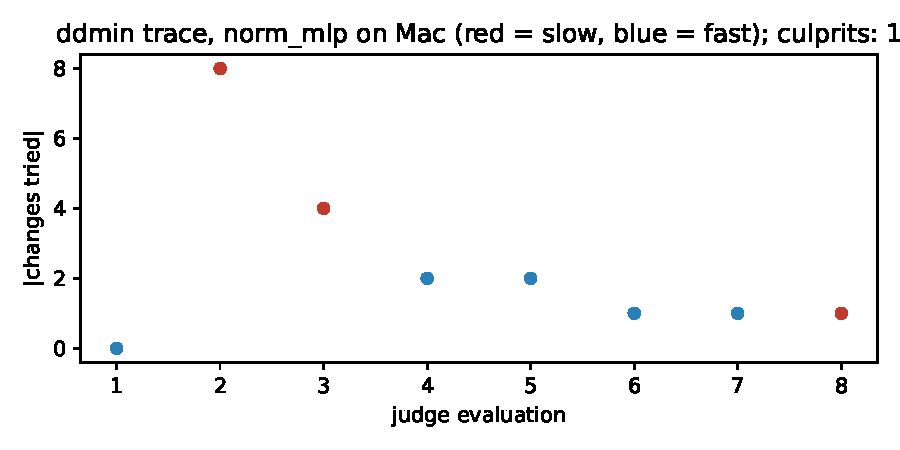
\includegraphics[width=0.7\linewidth]{figures/trace_norm_mlp_mac.pdf}\caption{ddmin search trace for norm\_mlp (Mac (M4 Pro, 8 threads)): each point is one judge evaluation.}\end{figure}}{}

\subsection*{resnet18 on the Mac (M4 Pro, 8 threads): verdict \emph{single}}
The slow state differs from the fast state in 6 switches. Fast 26.205~ms vs.\ slow 29.119~ms (+11.1\%); $\tau$ = 0.576~ms. ddmin needed 5 judge evaluations (versus 6 for leave-one-out, 15 for all pairs) and returned the culprit set \code{-lowering/layout\_\allowbreak{}optimization}. A single change reproduces the whole slowdown. \textbf{Kernel-level explanation.} fused kernels 14 $\rightarrow$ 12, extern calls 21 $\rightarrow$ 21, intermediate bytes 30,052,352 $\rightarrow$ 6,470,912. Kernels lost: \code{cpp\_\allowbreak{}fused\_\allowbreak{}\_\allowbreak{}native\_\allowbreak{}batch\_\allowbreak{}norm\_\allowbreak{}legit\_\allowbreak{}no\_\allowbreak{}training\_\allowbreak{}add\_\allowbreak{}convolution\_\allowbreak{}relu} ($\times$7), \code{cpp\_\allowbreak{}fused\_\allowbreak{}\_\allowbreak{}native\_\allowbreak{}batch\_\allowbreak{}norm\_\allowbreak{}legit\_\allowbreak{}no\_\allowbreak{}training\_\allowbreak{}convolution\_\allowbreak{}max\_\allowbreak{}pool2d\_\allowbreak{}with\_\allowbreak{}indices\_\allowbreak{}relu}, \code{cpp\_\allowbreak{}fused\_\allowbreak{}convolution}. Kernels gained: \code{cpp\_\allowbreak{}fused\_\allowbreak{}\_\allowbreak{}native\_\allowbreak{}batch\_\allowbreak{}norm\_\allowbreak{}legit\_\allowbreak{}no\_\allowbreak{}training\_\allowbreak{}add\_\allowbreak{}relu} ($\times$6), \code{cpp\_\allowbreak{}fused\_\allowbreak{}\_\allowbreak{}native\_\allowbreak{}batch\_\allowbreak{}norm\_\allowbreak{}legit\_\allowbreak{}no\_\allowbreak{}training\_\allowbreak{}max\_\allowbreak{}pool2d\_\allowbreak{}with\_\allowbreak{}indices\_\allowbreak{}relu}. 
\begin{table}[h]\centering\small
\begin{tabular}{lp{0.62\linewidth}}\toprule
field & value \\\midrule
\textbf{model} & resnet18 (Chideras-MacBook-Pro-2) \\
judge & timing (median\_ms) \\
fast reference & 26.118 ms, $\tau$ = 0.576 ms (2.2\%) \\
slow state & 29.119 ms \\
candidate changes & 6 \\
judge evaluations & 5 \\
verdict & single \\
culprits & \code{-lowering/layout\_\allowbreak{}optimization} \\
kernels fast $\rightarrow$ culprits & 14 $\rightarrow$ 12 \\
extern calls & 21 $\rightarrow$ 21 \\
intermediate bytes & 30,052,352 $\rightarrow$ 6,470,912 \\
median ms & 26.205 $\rightarrow$ 29.007 \\
\bottomrule\end{tabular}
\caption{Attribution summary, resnet18.}
\end{table}
\IfFileExists{figures/trace_resnet18_mac.pdf}{\begin{figure}[h]\centering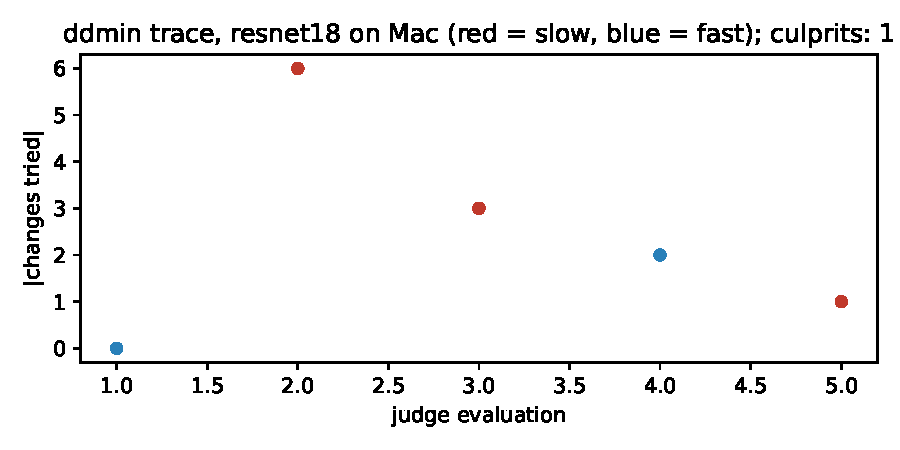
\includegraphics[width=0.7\linewidth]{figures/trace_resnet18_mac.pdf}\caption{ddmin search trace for resnet18 (Mac (M4 Pro, 8 threads)): each point is one judge evaluation.}\end{figure}}{}

\subsection*{attention\_block on the VM (Xeon, 4 threads): verdict \emph{single}}
The slow state differs from the fast state in 63 switches. Fast 7.621~ms vs.\ slow 8.265~ms (+8.4\%); $\tau$ = 0.162~ms. ddmin needed 8 judge evaluations (versus 63 for leave-one-out, 1953 for all pairs) and returned the culprit set \code{+joint/joint\_\allowbreak{}graph.\allowbreak{}patterns/\_\allowbreak{}sfdp\_\allowbreak{}pattern\_\allowbreak{}11\_\allowbreak{}inference}. A single change reproduces the whole slowdown. \textbf{Kernel-level explanation.} fused kernels 4 $\rightarrow$ 1, extern calls 4 $\rightarrow$ 3, intermediate bytes 11,591,680 $\rightarrow$ 4,198,400. Kernels lost: \code{cpp\_\allowbreak{}fused\_\allowbreak{}\_\allowbreak{}softmax\_\allowbreak{}abs\_\allowbreak{}all\_\allowbreak{}amax\_\allowbreak{}div\_\allowbreak{}eq\_\allowbreak{}mul\_\allowbreak{}ne\_\allowbreak{}sub\_\allowbreak{}view}, \code{cpp\_\allowbreak{}fused\_\allowbreak{}clone\_\allowbreak{}split\_\allowbreak{}transpose\_\allowbreak{}view}, \code{cpp\_\allowbreak{}fused\_\allowbreak{}clone\_\allowbreak{}transpose\_\allowbreak{}view}. Extern calls lost: \code{extern\_\allowbreak{}kernels.\allowbreak{}bmm} ($\times$2); gained: \code{torch.\allowbreak{}ops.\allowbreak{}aten.\allowbreak{}\_\allowbreak{}scaled\_\allowbreak{}dot\_\allowbreak{}product\_\allowbreak{}flash\_\allowbreak{}attention\_\allowbreak{}for\_\allowbreak{}cpu}. 
\begin{table}[h]\centering\small
\begin{tabular}{lp{0.62\linewidth}}\toprule
field & value \\\midrule
\textbf{model} & attention\_block (fa26-cs598a-010) \\
judge & timing (median\_ms) \\
fast reference & 7.650 ms, $\tau$ = 0.162 ms (2.1\%) \\
slow state & 8.265 ms \\
candidate changes & 63 \\
judge evaluations & 8 \\
verdict & single \\
culprits & \code{\_\allowbreak{}sfdp\_\allowbreak{}pattern\_\allowbreak{}11\_\allowbreak{}inference} \\
kernels fast $\rightarrow$ culprits & 4 $\rightarrow$ 1 \\
extern calls & 4 $\rightarrow$ 3 \\
intermediate bytes & 11,591,680 $\rightarrow$ 4,198,400 \\
median ms & 7.621 $\rightarrow$ 8.326 \\
\bottomrule\end{tabular}
\caption{Attribution summary, attention\_block.}
\end{table}
\IfFileExists{figures/trace_attention_block_vm.pdf}{\begin{figure}[h]\centering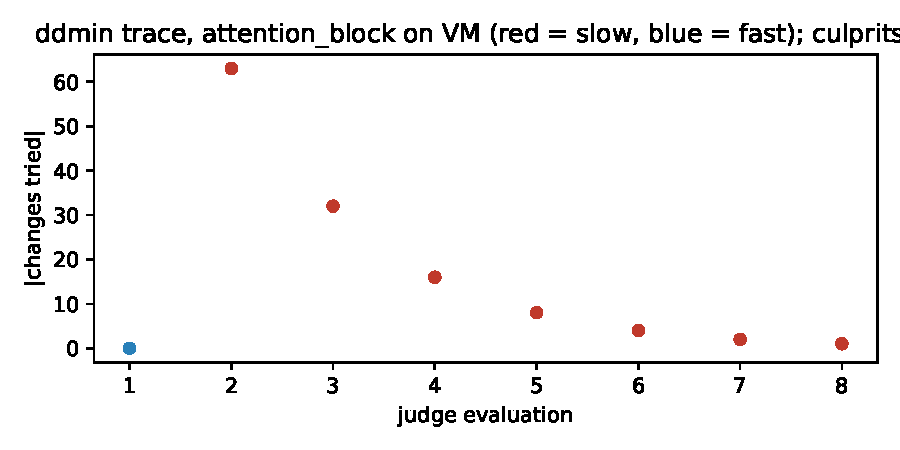
\includegraphics[width=0.7\linewidth]{figures/trace_attention_block_vm.pdf}\caption{ddmin search trace for attention\_block (VM (Xeon, 4 threads)): each point is one judge evaluation.}\end{figure}}{}%


\section{Status against the proposal and plan to the final report}
\begin{table}[h]\centering\small
\begin{tabular}{p{0.42\linewidth}p{0.5\linewidth}}\toprule
proposal item & status \\\midrule
1. Corpus (10--15 models) and a switch per rewrite rule, verified to change the graph &
  \textbf{Done.} 24 models registered, 269 switches, verification tool classifies each switch's effect per model. \\
2. Measurement harness: cached compiles, kernel and byte counters, timing with warm-up/trials, noise threshold &
  \textbf{Done} on the CPU backend; counters also parse Triton output (unit-tested). \\
3. Testing task 1: $\ge 30$ unit tests with planted slowdowns, counter and threshold tests &
  \textbf{Done, growing}: 100 %
tests (Table~\ref{tab:tests}). \\
4. Interim report: harness on 3--4 models with one clean attribution &
  \textbf{Done}: this report. \\
5. Attribution tool: ddmin over rule sets, timing judge, pair check, kernel-level diff &
  \textbf{Working first version}; needs more real-model case studies and a sensitivity study of $\tau$. \\
6. Testing task 2: full corpus, two largest models, repeatability across days and machines &
  \textbf{Started}: sweeps run on both machines; the largest models (ViT-B/16, Qwen2.5-0.5B) are registered but not yet measured. \\
7. Stretch: learned guards & Not started. \\
8. Final report, README, cleanup & README exists. \\
\bottomrule\end{tabular}
\end{table}

\paragraph{Risks and next steps.}
(1)~Timing noise on the shared 4-core VM is the main threat to attribution; the mitigation is the
measured $\tau$, the re-measure band, and running the sweeps on both machines. (2)~Most individual
rewrites are no-ops on a given model, so slowdowns on real models will come from a few rules
(attention fusion, freezing/oneDNN fusion, \code{decompose\_mm}, split/cat passes); the next sweeps
turn these opt-in families on in combination to look for pairs, as proposed. (3)~Decode graphs
should use a real KV cache. (4)~If GPU access appears, the same commands run with
\code{--device cuda} after a one-line change in the model builders.

\begin{thebibliography}{9}\small
\bibitem{zinenko} O. Zinenko et al. The MLIR Transform Dialect. arXiv:2409.03864, 2024.
\bibitem{vohra} A. Vohra et al. Mind the Abstraction Gap: Bringing Equality Saturation to Real-World ML Compilers. OOPSLA 2025.
\bibitem{taso} Z. Jia et al. TASO. SOSP 2019.
\bibitem{bisector} PyTorch. \code{torch/\_inductor/compiler\_bisector.py}, 2025.
\bibitem{zeller} A. Zeller and R. Hildebrandt. Simplifying and Isolating Failure-Inducing Input. IEEE TSE, 2002.
\bibitem{ansel} J. Ansel et al. PyTorch 2. ASPLOS 2024.
\end{thebibliography}
\end{document}
